\documentclass[oneside,a4paper,titlepage]{scrartcl} % Format fuer Titelseite und Dokument (Koma-Script)
\usepackage[ngerman]{babel}                         % Sprache
\usepackage[utf8]{inputenc}                         % Direkte Eingabe von Umlauten Dokument
\usepackage[T1]{fontenc}                            % Silbentrennung auch bei Woertern mit Umlauten
\usepackage{graphicx}                               % Bilder
\usepackage{listings}                               % Aufzaehlungen
\usepackage{xcolor}                                 % Farbgebung des Sourcodes
\usepackage{lmodern}                                % Formatierung des Sourcecodes
\usepackage{longtable}                              % Fuer mehrseitige Tabellen
\usepackage{booktabs}                               % Fuer mehrseitige Tabellen
\usepackage{colortbl}                               % Fuer farbige Zeilen/Reihen in Tabellen

% Formatierung fuer Tabellen
\usepackage{tabularx}
\newcolumntype{L}[1]{>{\raggedright\arraybackslash}p{#1}} % L fuer linksbuendig mit Breitenangabe
\newcolumntype{C}[1]{>{\centering\arraybackslash}p{#1}}   % C fuer zentriert mit Breitenangabe
\newcolumntype{R}[1]{>{\raggedleft\arraybackslash}p{#1}}  % R fuer rechtsbuendig mit Breitenangabe

% Fuer den automatischen Umbruch an einem Bindestrich, wie z.B. bei "Werkstueck-Sortieranlage", statt - die Zeichen "= verwenden

% Beginn des Dokuments
\begin{document}

% Titelseite aufbauen
\titlehead{\flushright}
\subject{Software Engineering II\\Wintersemester 2014/2015}
\title{Handbuch für PUCKMASTER 2000} 
\subtitle{ Praktikums-Gruppe: 2.3}

% Titelseite: Autoren aufbauen
\author{
\begin{small}
 \begin{tabular}{|l|l|c|L{6cm}|}
  \hline
  \rowcolor{lightgray}\textbf{Name} & \textbf{Vorname} & \textbf{Matrikel-Nr.} & \textbf{E-Mail}\\
  \hline
  \rowcolor{white}Kirstein & Katja & 2125137 & katja.kirstein@haw-hamburg.de\\
  \hline
  Kowalka & Anne-Lena & 2081899 & anne-lena.kowalka@haw-hamburg.de\\
  \hline
  Triebe & Marian & 2124897 & marian.triebe@haw-hamburg.de\\
  \hline
  Winter & Eugen & 2081992 & eugen.winter@haw-hamburg.de\\
  \hline
 \end{tabular}
\end{small}
}

% Titelseite mit Datum und Version erstellen und Seitenzahl bei 1 beginnen
\date{\today}
\maketitle

% Inhaltsverzeichnis anlegen
\thispagestyle{empty}
\tableofcontents
\newpage
\setcounter{page}{1}

\section{Einleitung}
\textbf{Sehr geehrter Kunde, sehr geehrte Kundin, \newline
wir gratulieren zum Erwerb einer PUCKMASTER 2000. 
Die Zukunft der Werkstücksortierung beginnt heute bei Ihnen!\newline
Mit dieser innovativen Anlage können Sie Werkstücke nach Größe und Typ sortieren - die verbaute Ampelanlage hilft Ihnen dabei!\newline
Im Vergleich zum PUCKMASTER 1000 gibt es folgende Verbesserungen : \newline
\begin{itemize}
    \item doppelte Bandgeschwindigkeit
    \item doppelte Anzahl von Werkstücken
    \item doppelt so genaue Höhenmessung
    \item doppelt so performante Software
\end{itemize}
Wir wünschen Ihnen viel Spaß mit Ihrer PUCKMASTER 2000!}

\newpage
\section{Allgemeine Sicherheitshinweise}
\textbf{\newline Die Werkstücksortieranlage wird aus technischen Gründen in der folgenden Dokumentation als Anlage bezeichnet.\newline}
\textbf{Technische Änderungen und Ergänzungen der      Beschreibung/Anleitung sind vorbehalten. \newline
Für den Inhalt wird keine Haftung übernommen, insbesondere für Schäden durch vorhandene, nicht 
vorhandene oder fehlerhafte Angaben. \newline
Weitergabe und Ergänzung dieser Beschreibung/ Betriebsanleitung sind nicht gestattet, soweit nicht    ausdrücklich genehmigt.\newline}
\textbf{Der Betreiber der Anlage ist verpflichtet, eine Betriebsanweisung für das Bedienungspersonal zu erstellen, um dieses vor Gefährdung der Gesundheit oder anderen sicherheitstechnischen Gefahren zu schützen. Außerdem ist der Betreiber verpflichtet, das Bedienungspersonal über die sichere und ordnungsgemäße Bedienung und den sachgerechten Betrieb der Anlage zu unterweisen.}
\newpage 

\section{Sicherheit}
\subsection{Allgemeines}
\textbf{Es ist darauf zu achten, dass die Anlage gemäß dieser Anleitung verwendet wird. Unsachgemäße Verwendung
kann zu unerwartetem Verhalten führen und sollte vermieden werden. Für Schäden, die aus unsachgemäßem Betrieb resultieren, haftet der Betreiber/Benutzer der Anlage.}

\subsection{Sicherheitsvorrichtungen}
\textbf{Die Anlage verfügt über diverse Vorrichtungen, um dem Benutzer Sicherheit zu gewähren:}

\subsubsection{Stoppen}
\textbf{Die Anlage kann jederzeit durch die Betätigung des Not-Aus-Buttons zum Stillstand gebracht werden.\newline
Nach einer Betätigung dieses Buttons müssen alle Werkstücke von beiden Bändern entnommen werden, sodass die Anlage neu gestartet werden kann.}

\subsubsection{Warnsignale}
\textbf{Die Sortierbänder verfügen über jeweils eine Ampel, über die der aktuelle Zustand des Sortierbands mitgeteilt wird.}

\newpage

\section{Beschreibung der Anlage}
\textbf{Die Anlage besteht aus zwei Fließbändern, die hintereinander aufgestellt werden und durch die jeweils zugehörige Software gesteuert werden.}
\subsection{Fließbandbestandteile}
\textbf{Die Fließbänder werden über jeweils eigene Motoren gesteuert. \newline
Jedes Fließband verfügt über mehrere Lichtschranken, über die die aktuelle Position des Werkstücks übermittelt wird. Diese Lichtschranken befinden sich an folgenden Positionen: am Fließbandeingang (B[0]), in der Höhenmessung (B[1]), in der Weiche (B[3]), in der Rutsche (B[6]) und am Fließbandausgang (B[7]). \newline
Desweiteren verfügt jedes Fließband über einen Höhensensor, über den die Höhe des Werkstücks ermittelt und ausgewertet wird. \newline
Außerdem gibt es eine Weiche (A[4]), die sich öffnet, sobald ein valides Werkstück den Weichenbereich passiert. In diesem Bereich befindet sich zudem ein Metallsensor (B[4]), der registriert, ob ein Werkstück Metall beinhaltet.\newline
Zur Kommunikation verfügen die zugehörigen GEME-Rechner über jeweils min. eine serielle Schnittstelle\newline }

\subsubsection{Portbeschreibung}
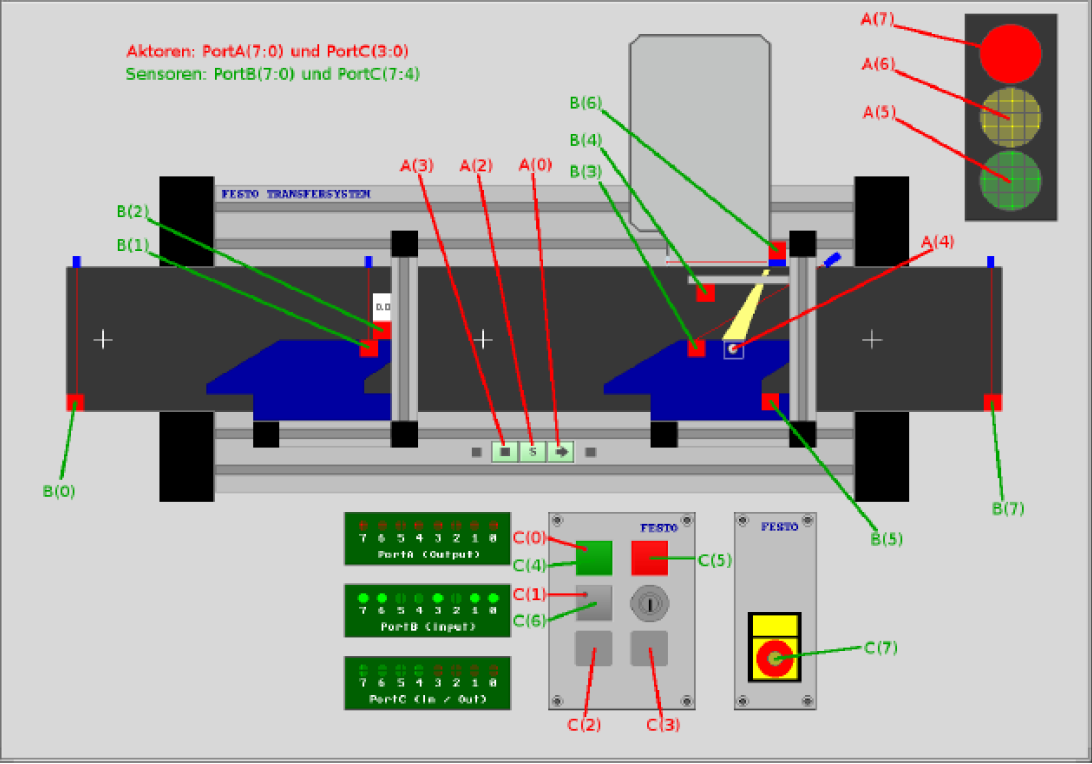
\includegraphics[scale=.5]{imgs/Portbeschreibung.PNG}
\newpage
\textbf{Die Ports ermöglichen die Ansteuerung der Aktorik bzw. das Auslesen der Sensorik.\newline}
\begin{itemize}
    \item Port A : Aktorik
    \begin{itemize}
        \item Bit 0-3 : Motorsteuerung
        \item Bit 4 : Weichensteuerung
        \item Bit 5-7 : Ampelsteuerung
    \end{itemize}
    \item Port B : Sensorik
    \begin{itemize}
        \item Bit 0 : Werkstück im Einlauf
        \item Bit 1 : Werkstück in Höhenmessung
        \item Bit 2 : Höhenmessung
        \item Bit 3 : Werkstück in Weiche
        \item Bit 4 : Metallsensor
        \item Bit 5 : Weiche offen oder geschlossen
        \item Bit 6 : Rutsche voll
        \item Bit 7 : Werkstück im Auslauf
    \end{itemize}
    \item Port C: : Ein-/Ausgabe
    \begin{itemize}
        \item Bit 0 : Start-LED
        \item Bit 1 : Reset-LED
        \item Bit 2 : Q1-LED
        \item Bit 3 : Q2-LED
        \item Bit 4 : Start-Button
        \item Bit 5 : Stop-Button
        \item Bit 6 : Reset-Button
        \item Bit 7 : Not-Aus-Button \newline
    \end{itemize}
\end{itemize}


\subsection{Werkstückdefinition}
\textbf{Es gibt folgende Werkstücktypen: }
\begin{itemize}
    \item zu flache Werkstücke (werden von Band eins aussortiert)
    \item Werkstücke mit valider Höhe, Bohrung und Metalleinsatz 
    \item Werkstücke mit valider Höhe, Bohrung, ohne Metalleinsatz 
\end{itemize}
\textbf{Es wird empfohlen, ausschließlich Werkstücke dieser Art auf die Fließbänder zu legen, um Beschädigungen der Anlage zu verhindern.}
\newpage

\section{Installation}
\textbf{Für den ordnungsgemäßen Betrieb werden zwei Fließbänder hintereinander aufgestellt.\newline
Die Ports der Fließbänder(A, B, C) werden mit den jeweiligen  Ports der GEME-Rechner verbunden und die Fließbänder werden an den Strom angeschlossen. \newline
Die seriellen Schnittstellen der beiden GEME-Rechner werden miteinander verbunden. \newline
Anschließend werden die Fließbänder eingeschaltet und auf den Rechnern wird die jeweilige Software gestartet.\newline
%TODO : Start-Button zum starten?
Die LED des Start-Buttons leuchtet, um dem Personal zu signalisieren, dass die Anlage betriebsbereit ist und gestartet werden kann.}
\newpage

\section{Betrieb}
\subsection{Normalbetrieb}
\textbf{Durch Betätigung des Start-Buttons wird die Anlage in den Normalbetrieb versetzt.\newline
Die grüne Signalleuchte leuchtet dauerhaft.\newline
Das Personal legt Werkstücke an den Anfang von Band eins. Dieses startet automatisch den Motor und beginnt mit der Aussortierung von zu kleinen Werkstücken. Hierbei ist darauf zu achten, dass die Werkstücke mit genügend Abstand (mindestens 5 cm) in richtiger Reihenfolge in die Eingangslichtschranke gelegt werden. \newline
Erreicht ein Werkstück das Ende von Band eins, wird es an Band zwei übergeben, sofern dieses frei ist. Andernfalls wartet das Werkstück am Ende von Band eins. \newline
Sobald das Werkstück das Ende von Band zwei erreicht hat, blinkt die gelbe Signalleuchte und das Werkstück muss vom Personal entnommen werden.\newline
Die zu dem jeweiligen Werkstück gehörigen Daten werden von dem zu Band zwei gehörigen Programm ausgegeben.}

\subsection{Fehlerbehandlung}
\subsubsection{Verschwinden von Werkstücken}
\textbf{Wird ein Werkstück während des laufenden Normalbetriebs von einem Sortierband entnommen, wird dies als Fehler festgestellt, die Sortierbänder stoppen und die roten Warnleuchten blinken schnell(1x pro Sekunde). Dieser Fehler muss mittels Reset-Button quittiert werden, sodass die roten Warnleuchten in ein dauerhaftes Leuchten übergehen. Abschließend wird der Normalbetrieb der Anlage über Betätigung des Start-Buttons fortgesetzt. }

\subsubsection{Hinzufügen von Werkstücken}
\textbf{Wird ein Werkstück während des laufenden Normalbetriebs "mitten"\ auf ein Sortierband gelegt, wird dies als Fehler festgestellt, die Sortierbänder stoppen und die roten Warnleuchten blinken schnell(1x pro Sekunde). Dieser Fehler muss mittels Reset-Button quittiert werden, sodass die roten Warnleuchten in ein dauerhaftes Leuchten übergehen. Das Personal muss anschließend das Werkstück, das hinzugefügt wurde, entfernen, sodass der Normalbetrieb der Anlage über Betätigung des Start-Buttons fortgesetzt werden kann.}

\subsubsection{Rutsche ist voll}
\textbf{Sobald die Rutsche eines Sortierbandes voll ist, wird dies als Fehler festgestellt, die Sortierbänder stoppen und die roten Warnleuchten blinken schnell. Dieser Fehler muss mittels Reset-Button quittiert werden, sodass die roten Warnleuchten in ein dauerhaftes Leuchten übergehen. Sobald das Personal die Rutsche min. ein Werkstück aus der vollen Rutsche entnommen hat, kann der Normalbetrieb über den Start-Button fortgesetzt werden. }

\subsubsection{Werkstück mit Bohrung nach unten auf Band eins}
\textbf{Sobald auf Band eins ein Werkstück mit der Bohrung nach unten erkannt wird, wird dieses Werkstück an das Bandende befördert. Sobald es die Lichtschranke durchbricht, stoppt das Band und die gelbe Signalleuchte blinkt. Das Personal muss das Werkstück wenden und zurück auf das Ende von Band eins legen, damit der Normalbetrieb fortsetzen kann. }

\subsubsection{Werkstücke in falscher Reihenfolge auf Band zwei}
\textbf{Wird von Band zwei eine falsche Reihenfolge der Werkstücke erkannt, wird ein betreffendes Werkstück zurück an den Anfang von Band zwei befördert und die gelbe Signalleuchte blinkt. Das Personal muss dieses Werkstück entnehmen, damit der Normalbetrieb fortsetzen kann.}

\subsubsection{Unquittierte Fehler}
\textbf{Wenn die Anlage einen Fehler registriert, der von selbst wieder verschwunden ist, blinkt die rote Signalleuchte langsam (1x pro 2 Sekunden). }

\subsubsection{Sonstige}
\textbf{Sollten während des Betriebes Fehler auftreten, deren Ursache unklar sind, empfiehlt es sich, den Resettaster zu betätigen, alle Werkstücke beider Sortierbänder zu entnehmen und die Anlage inklusive zugehöriger Software anschließend neuzustarten.}

\end{document}
}